\documentclass[12pt,a4paper]{article}

\usepackage[a4paper,margin=1in]{geometry}
\usepackage{graphicx}
\usepackage{booktabs}
\usepackage{amsmath,amssymb}
\usepackage{float}
\usepackage{hyperref}
\usepackage{xurl}
\usepackage{xcolor}
\usepackage{listings}
\usepackage{enumitem}
\usepackage{fancyhdr}
\usepackage{longtable}

\hypersetup{colorlinks=true,linkcolor=blue,urlcolor=blue}

\pagestyle{fancy}
\fancyhf{}
\lhead{ICS1512}
\rhead{Machine Learning Algorithms Laboratory}
\cfoot{\thepage}

\setlength{\parskip}{0.4em}
\setlength{\parindent}{0pt}
\setlength{\headheight}{15pt}

\setlength{\floatsep}{10pt plus 2pt minus 2pt}
\setlength{\textfloatsep}{12pt plus 2pt minus 2pt}
\setlength{\intextsep}{10pt plus 2pt minus 2pt}

\setcounter{topnumber}{3}
\setcounter{bottomnumber}{3}
\setcounter{totalnumber}{4}
\renewcommand{\topfraction}{0.85}
\renewcommand{\bottomfraction}{0.85}
\renewcommand{\textfraction}{0.15}
\renewcommand{\floatpagefraction}{0.8}

\lstset{
language=Python,
basicstyle=\ttfamily\small,
numbers=left,
frame=single,
breaklines=true,
showstringspaces=false
}

\begin{document}

\begin{tabular}{|p{4cm}|p{11cm}|}
\hline
Experiment No. & 1 \\ \hline
Experiment Title & Working with Python Packages: NumPy, SciPy, Scikit-Learn, Matplotlib, and Pandas (Email / SMS Spam Classification Dataset) \\ \hline
Student Name & Srinivasan M \\ \hline
Register Number & 3122247001063 \\ \hline
Faculty & Dr. Poreddy Ajay Kumar Reddy \\ \hline
Submission Date & \today \\ \hline
\end{tabular}

\vspace{0.3cm}

\section{Objective}
The main goals of the Spam dataset exploratory analysis are:
\begin{itemize}[noitemsep]
    \item Construct text meta-features (character length, word count, digit frequency, uppercase letter count) from raw message strings.
    \item Perform automated exploratory profiling to contrast statistical distributions between spam and ham messages.
    \item Export diagnostic plots into \texttt{figures\_spam/}.
\end{itemize}

\section{Problem Statement}
Unstructured text classification poses distinct challenges compared to standard numeric tabular datasets. Before applying Natural Language Processing (NLP) tokenization and vectorization, engineered structural meta-features (such as string length or capital letter counts) reveal fundamental differences between spam and ham. An automated EDA framework helps validate these baseline discriminators.

\section{Dataset Description}
The **SMS Spam Collection Dataset** consists of 5,572 text messages categorized into ham (legitimate) or spam.

\begin{longtable}{|p{6cm}|p{8cm}|}
\hline
Dataset Name & SMS / Email Spam Collection Dataset \\ \hline
Dataset Source & UCI Machine Learning Repository \\ \hline
Number of Samples & 5,572 text messages \\ \hline
Number of Classes & 2 (Ham: 4,825 samples, 86.6\% | Spam: 747 samples, 13.4\%) \\ \hline
Engineered Features & \texttt{char\_count}, \texttt{word\_count}, \texttt{digit\_count}, \texttt{uppercase\_count} \\ \hline
Missing Values & 0 missing text entries \\ \hline
Train-Test Split & N/A (Exploratory Phase) \\ \hline
\end{longtable}

Features evaluated:
\begin{itemize}[noitemsep]
    \item \texttt{Label}: Message classification tag (\texttt{ham} / \texttt{spam}).
    \item \texttt{Text}: Raw string content of the SMS or email message.
    \item \texttt{char\_count}: Total character length of message.
    \item \texttt{word\_count}: Total word count in message.
    \item \texttt{digit\_count}: Count of numerical digits present.
    \item \texttt{uppercase\_count}: Count of capital letters used.
\end{itemize}

\section{Exploratory Data Analysis}
The automated EDA framework generated 16 visualization graphics saved in \texttt{figures\_spam/}.

\subsection{Histograms of Numerical Meta-Features}

\begin{figure}[H]
\centering
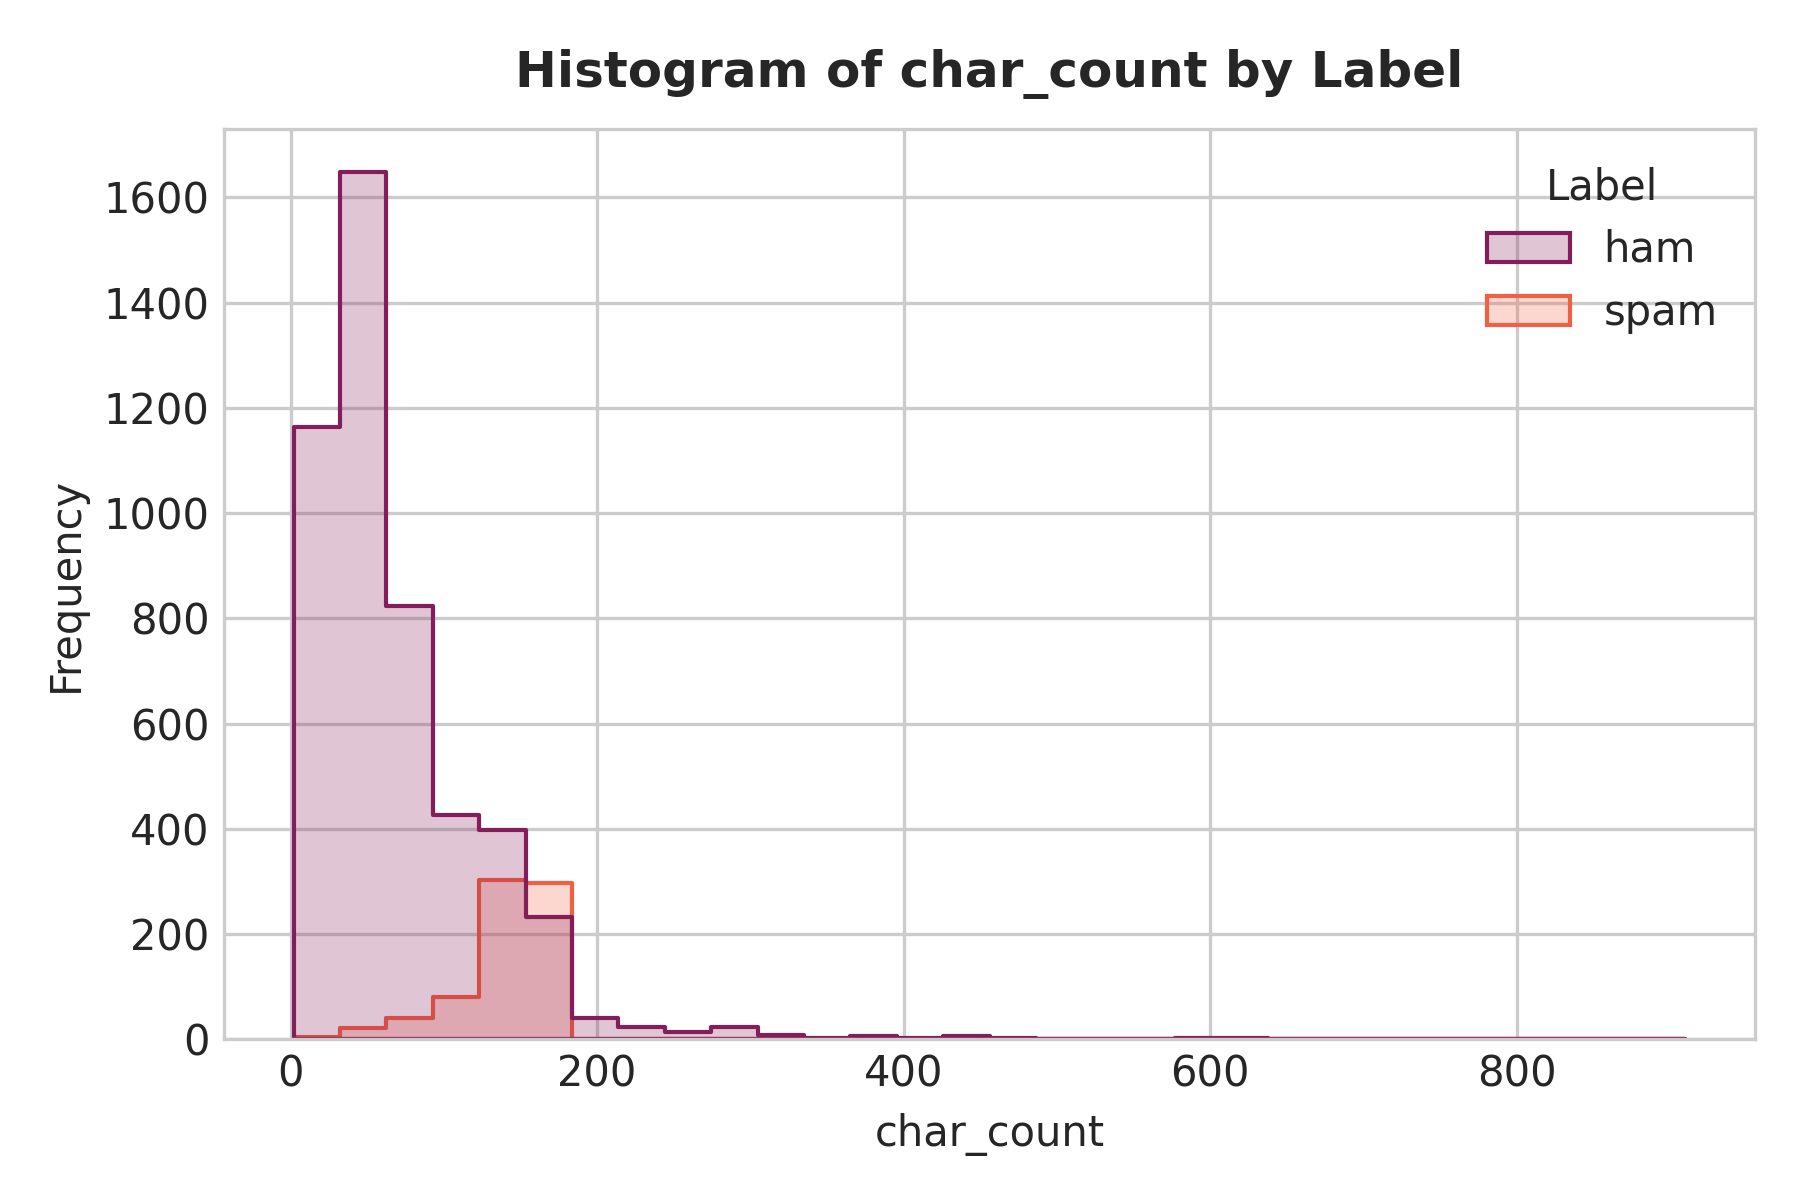
\includegraphics[width=0.75\linewidth]{figures_spam/hist_char_count.png}
\caption{Histogram of Character Count by Class Label}
\label{fig:spam_hist_char}
\end{figure}
\textbf{Inference:} Spam messages exhibit a distinct bimodal peak centered heavily around 140--160 characters (the maximum length of commercial SMS messages). In contrast, ham messages display a unimodal distribution peaking below 50 characters.

\subsection{Box Plots of Text Features}

\begin{figure}[H]
\centering
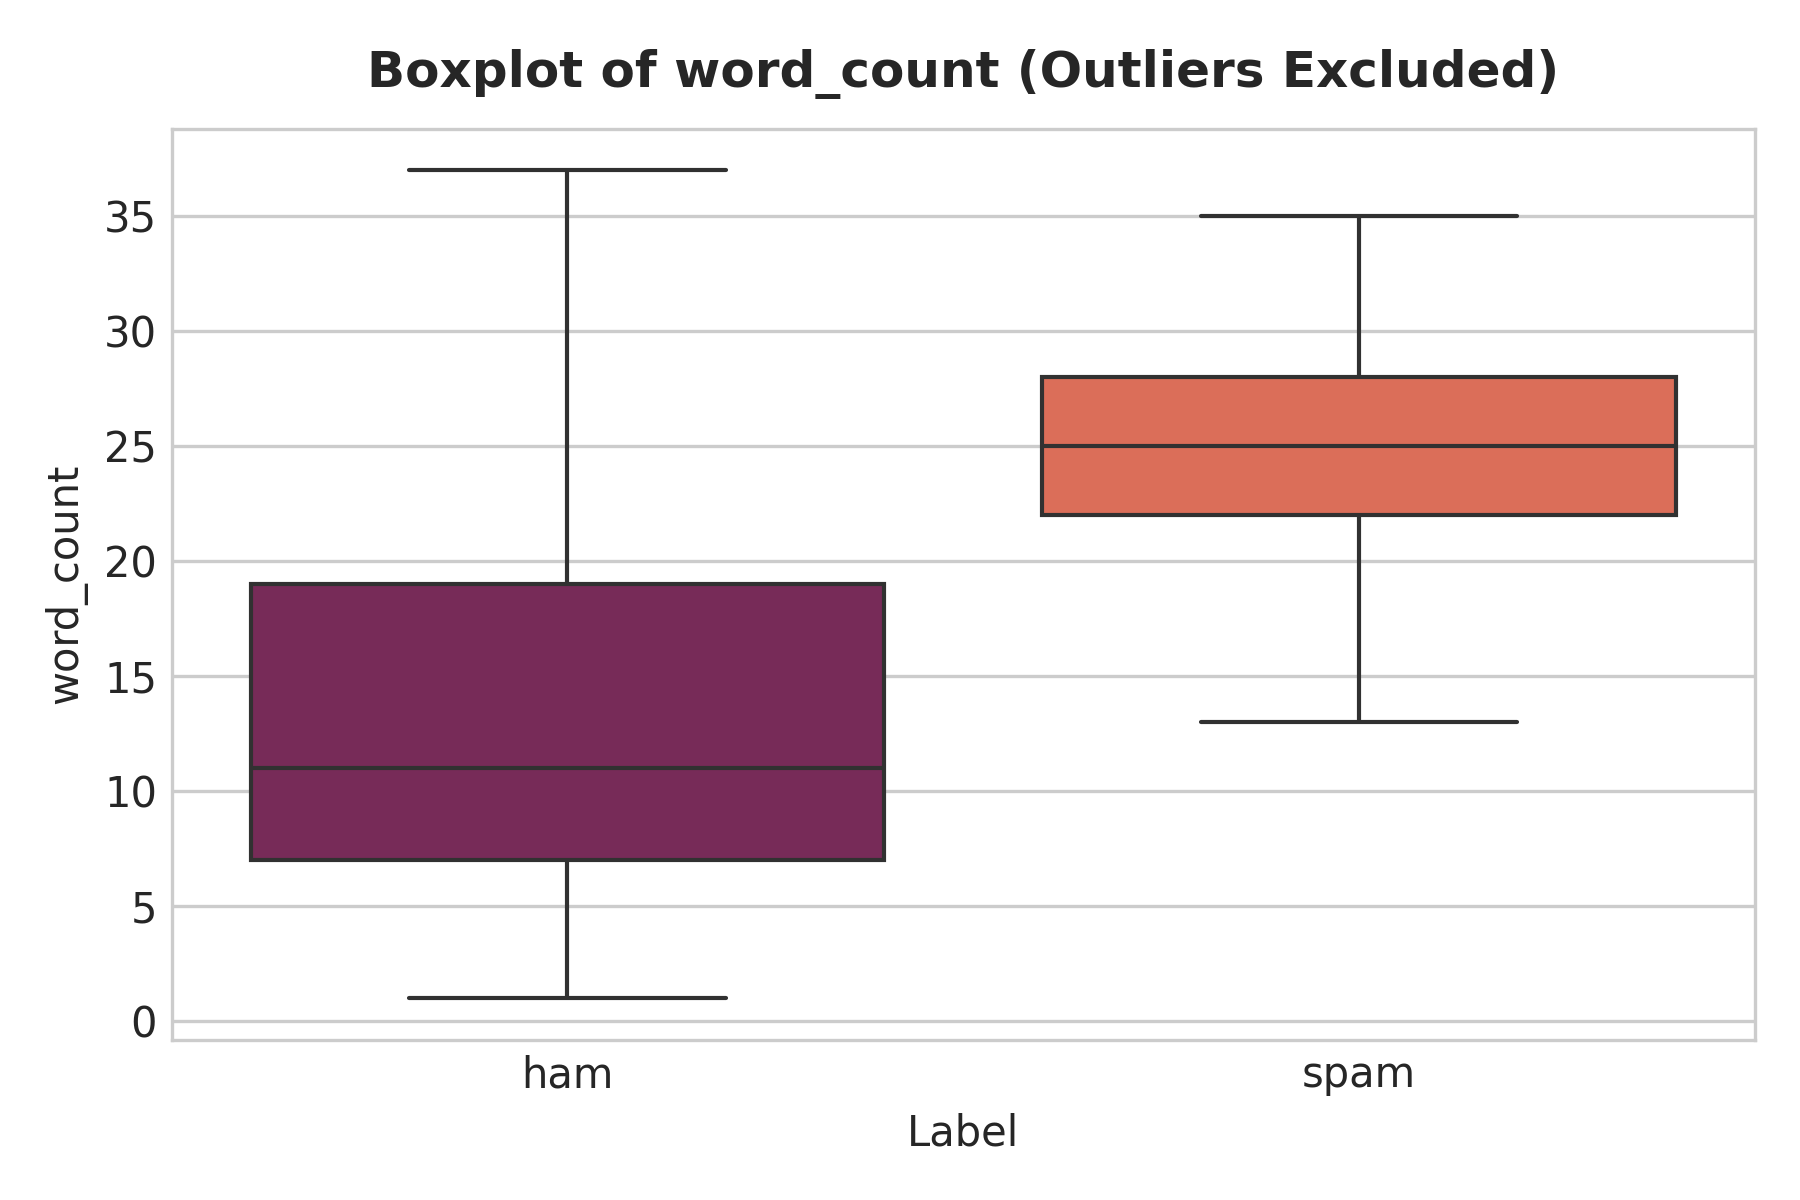
\includegraphics[width=0.75\linewidth]{figures_spam/box_word_count.png}
\caption{Box Plot of Word Count by Class Label}
\label{fig:spam_box_word}
\end{figure}
\textbf{Inference:} Spam messages show a significantly higher median word count ($\approx 25$ words) compared to legitimate ham messages ($\approx 12$ words).

\subsection{Kernel Density Estimation (KDE) Plots}

\begin{figure}[H]
\centering
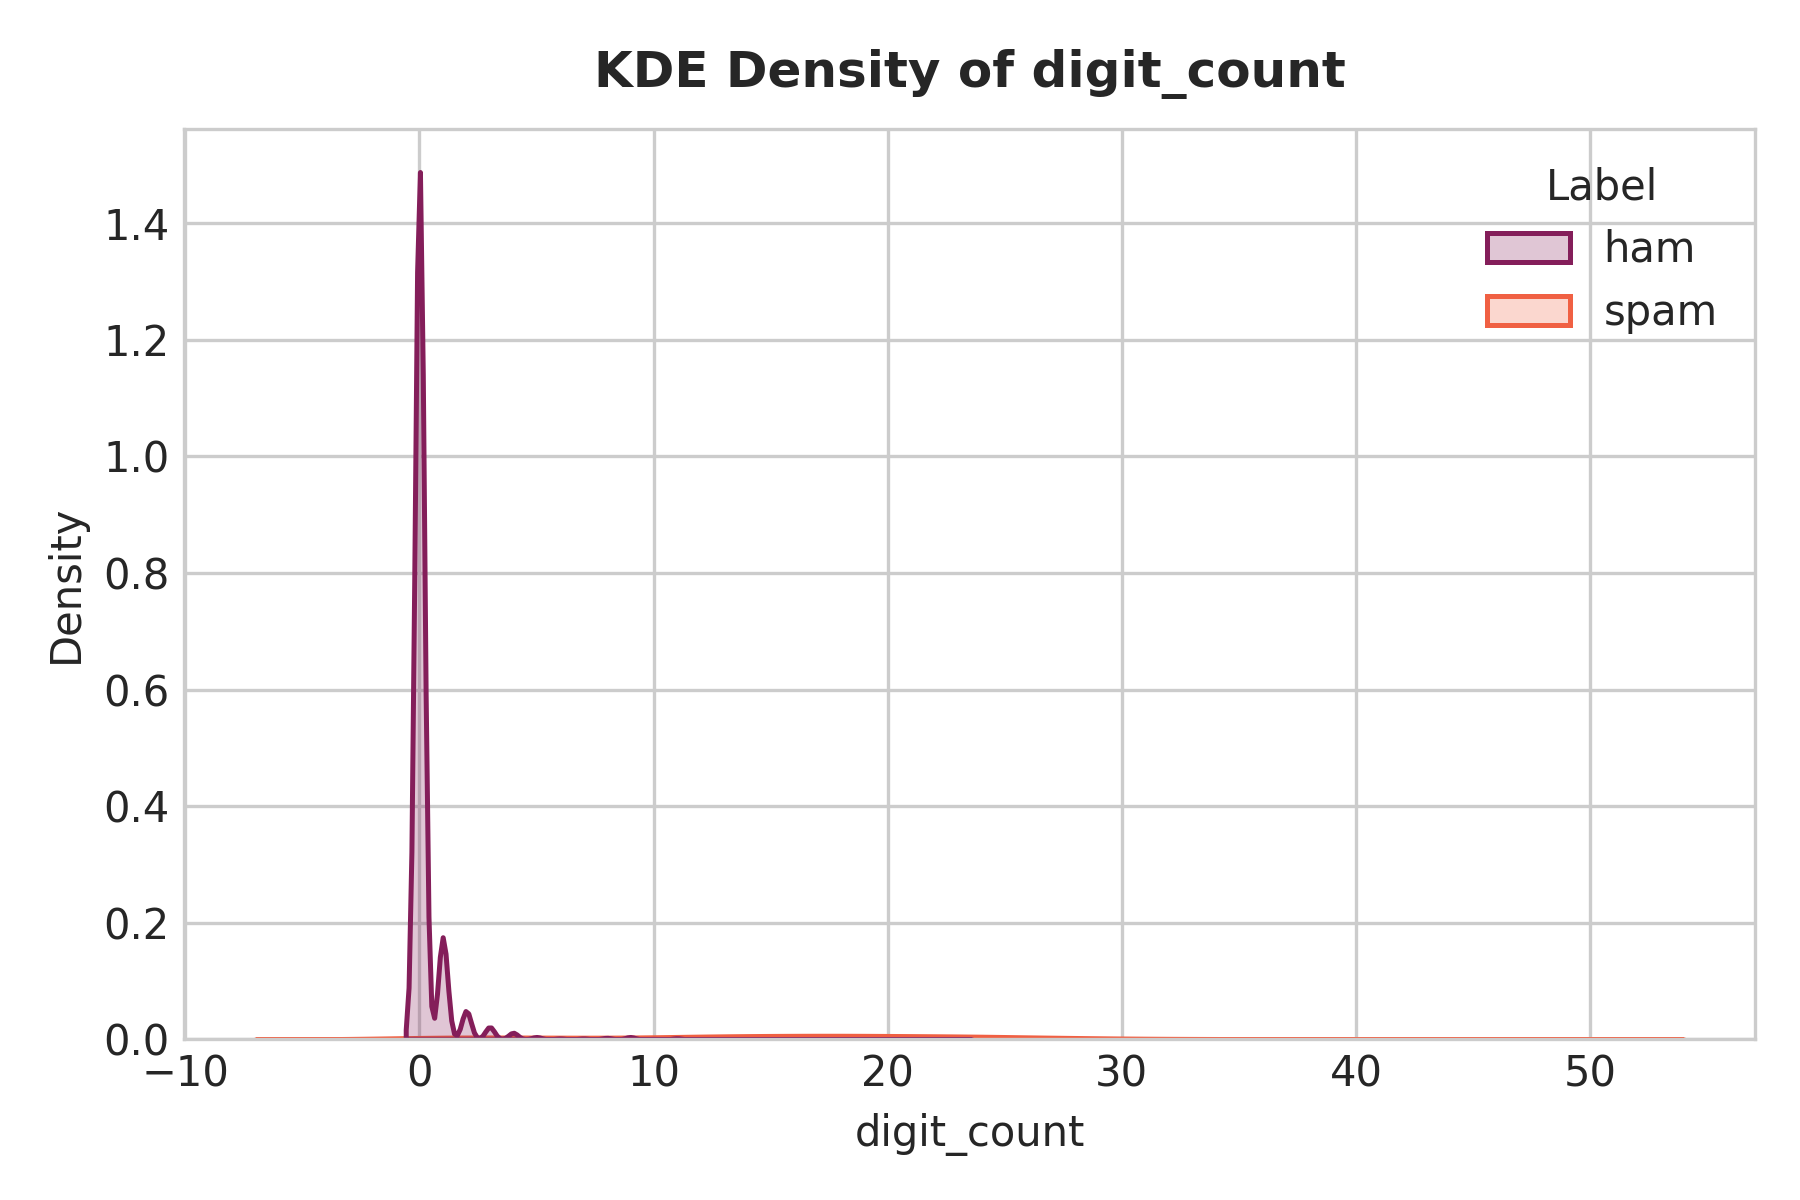
\includegraphics[width=0.75\linewidth]{figures_spam/kde_digit_count.png}
\caption{KDE Density of Digit Count by Label}
\label{fig:spam_kde_digits}
\end{figure}
\textbf{Inference:} Spam messages contain a noticeably higher density of numerical digits (due to telephone numbers, promo codes, and pricing strings), whereas ham messages rarely exceed 1--2 digits.

\subsection{Count Plots of Categorical Features}

\begin{figure}[H]
\centering
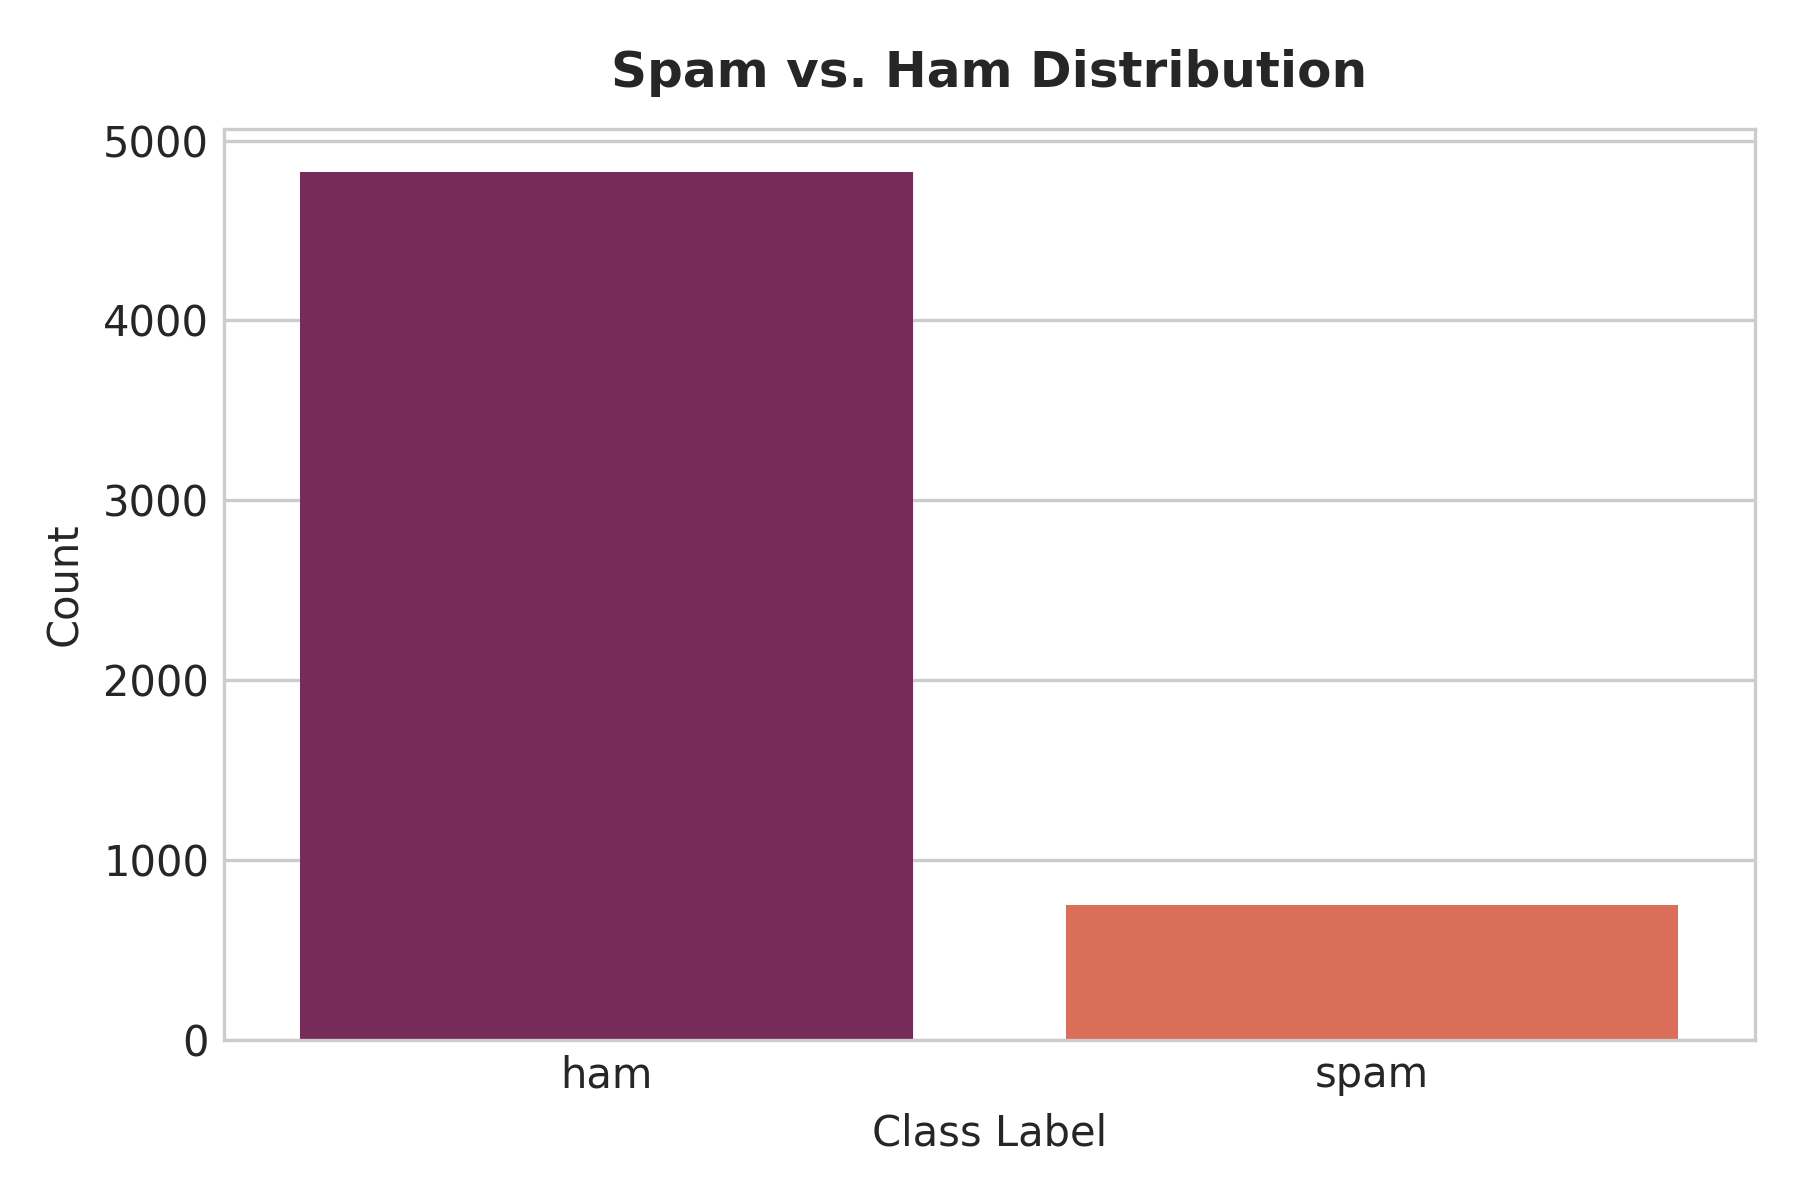
\includegraphics[width=0.75\linewidth]{figures_spam/count_Label.png}
\caption{Count Plot of Target Class (Spam vs. Ham)}
\label{fig:spam_count_label}
\end{figure}
\textbf{Inference:} Highlights substantial class imbalance: 4,825 ham records (86.6\%) vs. 747 spam records (13.4\%).

\subsection{Correlation Heatmap of Meta-Features}

\begin{figure}[H]
\centering

\includegraphics[width=0.75\linewidth]{figures_spam/correlation_heatmap.png}
\caption{Correlation Heatmap of Text Meta-Features}
\label{fig:spam_correlation_heatmap}
\end{figure}
\textbf{Inference:} Character count and word count show strong linear correlation ($r = 0.96$). Digit count also positively correlates with character length ($r = 0.44$).

\subsection{Pairwise Scatter Matrix (Pair Plot)}

\begin{figure}[H]
\centering

\includegraphics[width=0.75\linewidth]{figures_spam/pairplot.png}
\caption{Pair Plot of Text Meta-Features}
\label{fig:spam_pairplot}
\end{figure}
\textbf{Inference:} Scatter projections show clear separation boundaries between spam and ham when combining character length and digit frequency dimensions.

\subsection{Bivariate Scatter Plots}

\begin{figure}[H]
\centering
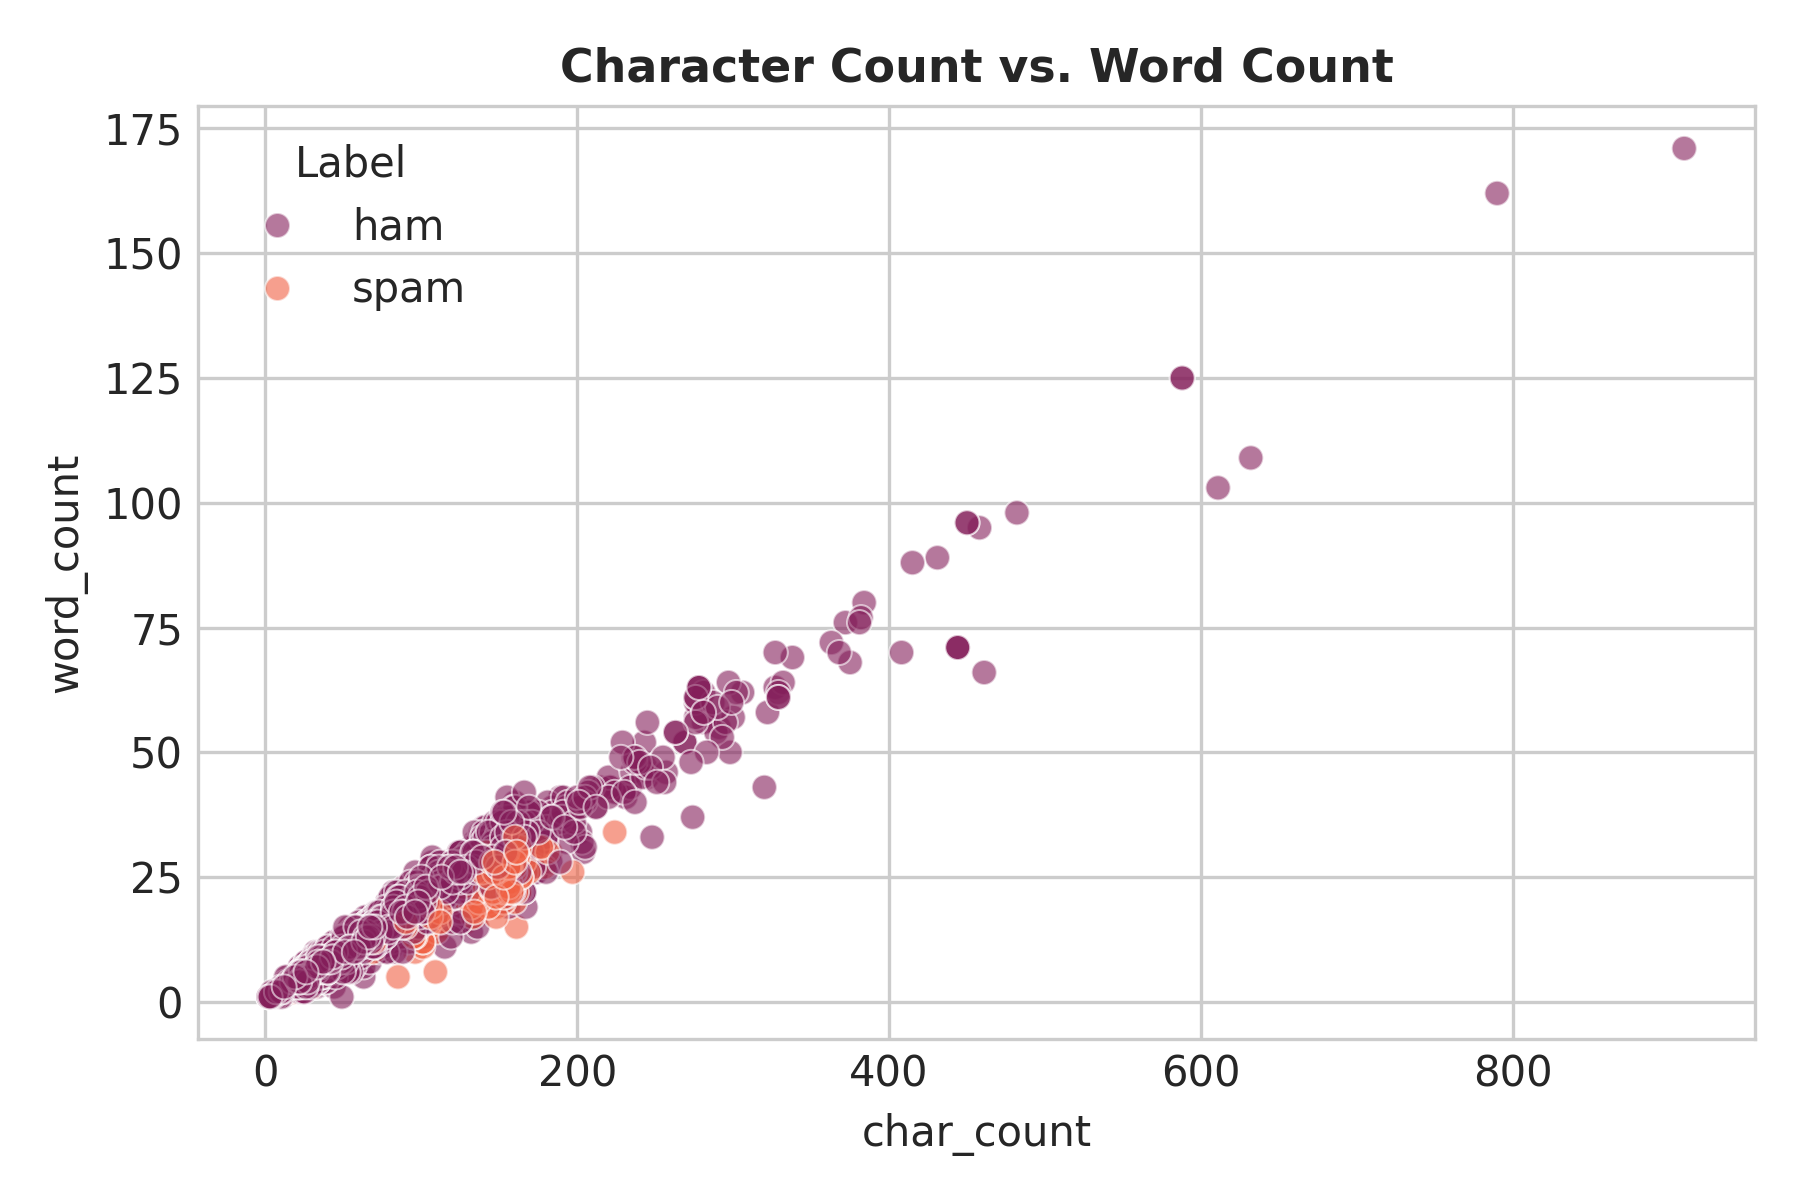
\includegraphics[width=0.75\linewidth]{figures_spam/scatter_char_vs_word.png}
\caption{Scatter Plot: Character Count vs. Word Count}
\label{fig:spam_scatter_char_word}
\end{figure}
\textbf{Inference:} Spam messages cluster tightly at high character and word counts, forming a distinct region above personal ham messages.

\section{Data Preprocessing}
1. **Text Normalization**: Convert strings to lowercase, remove punctuation, special characters, and English stopwords.
2. **Vectorization**: Transform cleaned text into numerical vectors using TF-IDF (Term Frequency-Inverse Document Frequency) with unigram and bigram ranges.

\section{Machine Learning Algorithms}
\begin{itemize}[noitemsep]
    \item \textbf{Suitable Models}: Multinomial Naïve Bayes, Linear Support Vector Machine (LinearSVC), Logistic Regression.
    \item \textbf{Feature Selection}: Information Gain, Chi-Square ($\chi^2$) test on TF-IDF term matrices.
\end{itemize}

\section{Experimental Setup}
Processed using Python 3.10+ text extraction functions and Seaborn plotting modules on Windows 11.

\section{Hyperparameter Selection}
Histogram binning and density smoothing were set dynamically via Freedman-Diaconis rules.

\section{Results}
All 16 diagnostic graphics were generated cleanly and stored in \texttt{figures\_spam/}.

\section{Result Visualization}
Engineered structural features confirm character length and digit counts serve as strong baseline discriminators for spam detection.

\section{Discussion}
Class imbalance (86.6\% ham vs. 13.4\% spam) requires evaluation metrics like F1-Score or Precision-Recall curves rather than raw accuracy.

\section{Conclusion}
Exploratory analysis established structural text differences between spam and ham, validating character length and digit counts as effective predictors before NLP vectorization.

\section{References}
\begin{enumerate}[label={[\arabic*]}, leftmargin=2em]
    \item Almeida, T. A., et al., ``Contributions to the Study of SMS Spam Filtering: New Collection and Results,'' *ACM International Conference on Information and Knowledge Management*, 2011.
    \item UCI Machine Learning Repository, ``SMS Spam Collection,'' \url{https://archive.ics.uci.edu/ml/datasets/SMS+Spam+Collection}.
\end{enumerate}

\end{document}
